\documentclass[12pt,twoside,a4paper, notitlepage]{article}%,a4paper

% Establim el format de la pàgina:
\usepackage{fancyhdr}
%\usepackage[a4paper]{geometry}
\usepackage[left=2cm,right=2cm,top=1.5cm, bottom=2cm]{geometry}
\setlength{\parskip}{0.2cm}
\usepackage[T1]{fontenc}
\usepackage[utf8]{inputenc}
\usepackage[catalan]{babel}
\usepackage{newunicodechar}
\newunicodechar{Ŀ}{\L.}
\newunicodechar{ŀ}{\l.}
\usepackage{siunitx}
\usepackage{amsmath}
%\usepackage{adjustbox}
%\usepackage{tabularx}
\usepackage{mathtools}
\usepackage{graphicx}
\usepackage{color}
\usepackage{caption}
\usepackage{subcaption}
\usepackage[colorlinks=true,urlcolor=blue,linkcolor=blue,citecolor=blue]{hyperref}
%\usepackage{booktabs} %Publication quality tables in LaTeX.
%\usepackage{pdflscape}
\usepackage{attachfile}
\usepackage{todonotes}
\usepackage{pdfpages}

\usepackage{sagetex}
\usepackage{color}
\definecolor{gris}{RGB}{220,220,220}

\author{Casimiro Victoria Castillo}


\begin{document}

%\title{}
%\author{}
%\date{}
%\date{}607123000
%\maketitle 
%\begin{titlepage}
%  \vspace*{4cm}
%  {\fontsize{28}{34}\selectfont\bfseries Fonons y espectroscòpia Raman en semiconductors bidimensionals}
%  \hfill
  % Logo
  %\includegraphics[height=2cm]{example-image-a} \\
  % Línea gris
%  {%\color{gris}
%  \hrule}
  %\Large{\itshape Subtítulo}
%  \vfill
%  {\large Casimiro Victoria Castillo \hfill 11 de Abril de 2021}
%\end{titlepage}

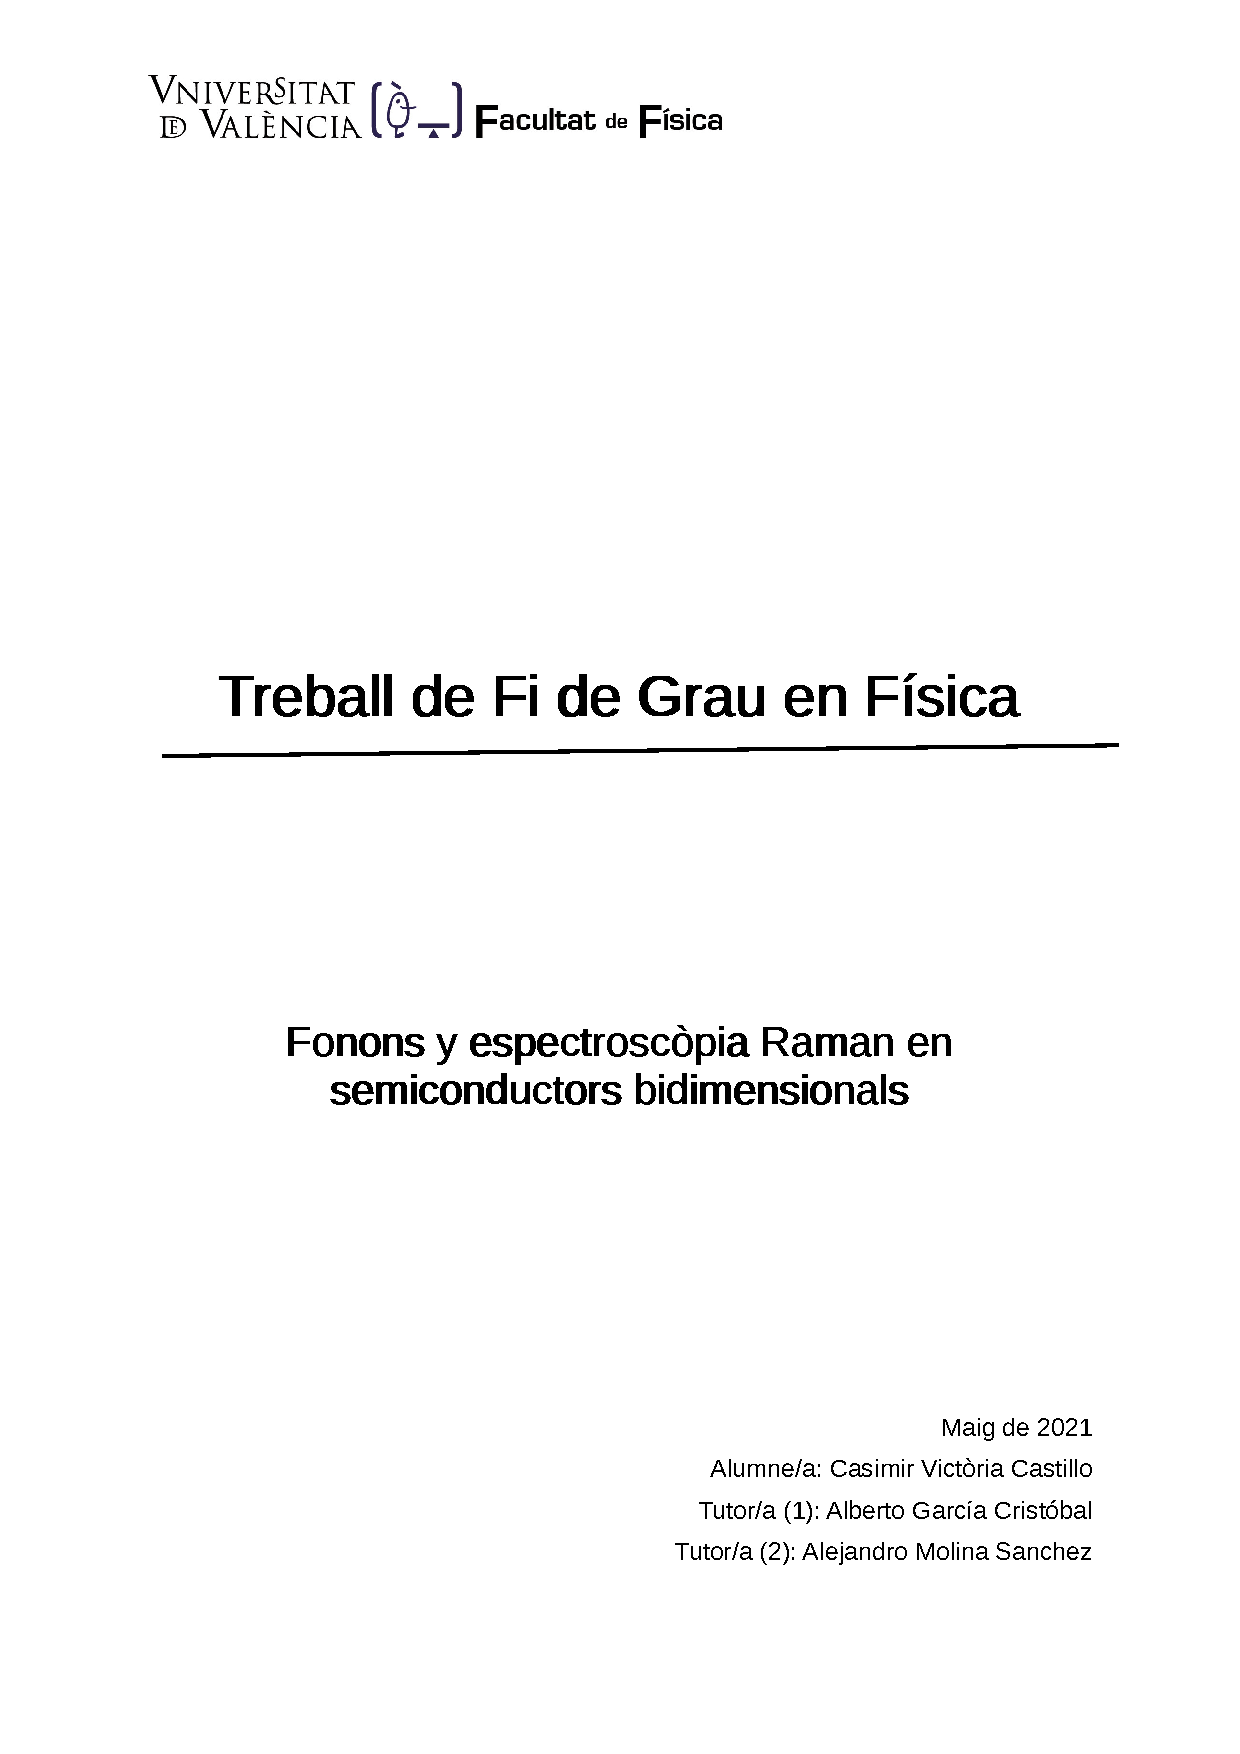
\includepdf{./Altres/portada_tfg_casimir.pdf}

\begin{abstract}
  Els materials bidimensionals ($2D$) com el grafè són de gran interès tant per les seues propietats físiques exclusives com per les seues aplicacions potencials. L'estudi de la dinàmica de la xarxa cristallina (\textit{fonons}) d'estos materials és un requisit previ per entendre la seua estabilitat estructural i propietats tèrmiques, així com les seues propietats de transport i òptiques.   


  Este Treball de Fi de Grau consisteix en la computació dels modes vibracionals de materials semiconductors 2D y la seua correlació amb els observables rellevants per a la interpretació dels experiments de dispersió de la llum.
\end{abstract}

\textit{Nota: s'ajunta el codi font del document: \attachfile[author=Casimir]{TFG-Casimir.tex}}

\newpage

\section{Introducció}

\todo[inline]{Per ara sols són algunes idees a desenvolupar}

\subsection{Model de BORN i VON KARMAN}
- Explicar el \textbf{model de  Born y  Von Karman (1921}), tal y com ve en \cite{Balkanski_2000} \cite{brueesch82_phonon} (pàgina 4).


\subsection{Aproximació adiabàtica}
Desprès explicar que fent ús de l'\textbf{aproximació adiabàtica}, podem, sempre que siga vàlida tal aproximació -explicar quan ho és- considerar els nuclis iònics y els electrons de valència com constituents del sòlid independents, de manera que podem escriure l'energia potencial (o el Hamiltonià) como una suma de les distintes contribucions.
  
\subsection{Aproximació armònica}
Passar a descriure l'\textbf{aproximació harmònica}: escriure el potencial, les equacions de moviment de Lagrange, y passar d'estes equacions de moviment en l'espai de posiciones al problema de valors propis de la matriu dinàmica en l'espai de vectores de onda (o moments).

Les vibracions reticulars estan regides per les forces que experimenten els àtoms quan es desplacen de la seua posició d'equilibri. La primera hipòtesi és que cada àtom té una posició d'equilibri en el cristall, y considerarem que estos àtoms vibren amb una amplitud menuda (en comparació amb la distància interatòmica) al voltant d'aquesta, de manera que el sòlid es troba en estats que corresponen al que macroscòpicament es coneix com \textit{la regió de comportament e\l.làstic lineal}, on es verifica la llei de Hooke.

Podem per tant aproximar l'energia potencial de interacció pel terme armònic del seu desenvolupament en sèrie de potencies del despla\c{c}ament ....


- Explicar el concepte de fonó i la seua importància: Un fonó és un mode de vibració quantitzat que té lloc en una xarxa cristallina. Els fonons tenen una gran importància en moltes propietats físiques dels sòlids. Los fonons son una version mecano-quàntica dels modes normals de vibració de la mecànica clàssica, on cada par de la xarxa osci\l.la amb la mateixa freqüència. Aquests modes normals són importants perquè qualsevol moviment vibracional de la xarxa pot descriure's com una superposició de modes normals de distinta freqüència, en este sentit són la base de les vibracions de la xarxa.

- Explicar també que una vegada descrit el cristall en l'espai de posicions tenim que descriure la xarxa cristallina en l'espai de moments ...

- Una vegada conclosa la introducció teòrica general, descriure el cristall de BN monocapa (xarxa cristallina, base, xarxa en l'espai $2\pi\text{-recíproc}$.

- Passar a construir la matriu dinàmica a partir del tensor de constants de for\c{c}a (cite Balkanski 2000) en coordenades cartesianes, tenint en compte que degut a la simetria del cristal la matriz de constantes de fuerza (y su transformada de Fourier, la matriz dinámica), té que complir certes relacions (forma de la matriz, elementos nulos, relación entre elementos, ...), cite aizawa90 bond soften monol graph formed (en el apèndix). 


\subsection{Xarxa recíproca. Primera zona de Brillouin.}
Donada una terna de vectors base primitius, $p_i$, de la xarxa cristalina en l'espai de posicion, la condició:

\begin{equation}
\label{eq:rec1}
\vec p_i\cdot\vec p_j^{*}=\delta_{ij}
\end{equation}
on $\delta_{ij}$ és la delta de Kronecker, pot considerar-se un sistema d'equacions que defieix una altra terna de vectors $p_j^*$. La solució de l'equació (\ref{eq:rec1}) és

\begin{equation}
\label{eq:rec2}
\vec p_1^*=\frac{\vec p_2\times\vec p_3}{\vec p_1\cdot(\vec p_2\times\vec p_3)},\quad \vec p_2^*=\frac{\vec p_3\times\vec p_1}{\vec p_1\cdot(\vec p_2\times\vec p_3)}, \quad \vec p_3^*=\frac{\vec p_1\times\vec p_2}{\vec p_1\cdot(\vec p_2\times\vec p_3)}
\end{equation} 

Els \textit{vectors recíprocs} $\vec p_j^{*}$ són els vectors d'una altra xarxa cristallina coneguda com \textit{xarxa recíproca}. Els  vectors recíprocs, i els vectors de translació cristallina recíprocs, tenen dimendions de inversa de longitut i es representen en l'\textit{espaci recíproc} o de números d'ona. \textbf{Les xarxes cristallines real y recíproca són dues descripcions equivalents del matexi sistema físic: el sòlido cristallí} que s'està estudiant.


Tenim que tindre present que l'espai $2\pi-$ recíproc és el fonamental en l'estudi de la Física de l'Estado Sòlid ja que els estats de les partícules i les interaccions físiques de interés es descriuen en l'espai de vectors d'ona.

Podem interpretar que 

\begin{equation}
\label{eq:rec3}
\vec K_{h_1h_2h_3}=2\pi\left(h_1\vec a_1^{*}+h_2\vec a_2^{*}+h_3\vec a_3^{*}\right)
\end{equation}

són els vectors de traslació cristallina que defineixen una xarxa cristallina en aquest espai $2\pi$-recíproc (sóls es diferencia de l'espai recíproc en un factor d'escala $2\pi$). En térmes físics, l'espai $2\pi$-recíproco és l'/espai de vectors d'ona/ $\vec k$, i a falta d'un factors d'escala $\hbar$, coincide amb l'espai de moments  $\vec p=\hbar\vec k$. 

\subsubsection{Ce\l.les de Wigner-Seitz (WS) y primera zona de Brillouin (ZB)}
Para descrire la xarxa 2$\pi$-recíproca, emprarem el criteri de \textit{Wigner-Seitz}. Las \textit{ce\l.les de Wigner-Seitz} estan centradas en un nuc de la xarxa i es defineixen com la regió més pròxima a un nuc (el del centre de la ce\l.la) que a quasevol altre. Per determinar la seua forma, partim d'un nuc qualsevol com a origen, construim els segments que uneixen este nuc amb els seus veïns i es tracen els plans que bissecten cadascun d'estos segments: la ce\l.la de WS és la ce\l.la de menor volumn al voltant de l'origen que està delimitadda per estos plans (rectes en el caso d'una xarxa bidimensional).

Notem que en l'espai de $\vec k$ emprarem ce\l.les unitat de WS mentre que en l'espai de posicions sempre emprem ce\l.les unitat de Bravais.
La ce\l.la de WS de la xarxa $2\pi$-recíproca es coneix com \textbf{primera zona de Brillouin} (ZB)

\newpage
\subsection{Matriu dinàmica}

La matriu dinàmica és la magnitud central de la dinàmica reticular: les freqüències dels fonons es calculen a partir dels valors propis de la matriu dinàmica:

\begin{equation}
\sum_{\alpha\prime}D_{\alpha\alpha\prime}\cdot\vec e_{\alpha\prime}(\vec q)=\omega^{2}\vec e_{\alpha}(\vec q)
\end{equation}   

Per tant, les freqüències $\omega$ com funció del vector d'ones $\vec q$ del fonó són solució de l'equació secular:

\begin{equation}
\det\left|\frac{1}{\sqrt{M_\alpha M_{\alpha\prime}}}D^{ij}_{\alpha\alpha\prime}\left(\vec q\right)-\omega^2\left(\vec q\right)\right|=0 
\end{equation}

on $M_{\alpha}$ es la massa de l'àtom $\alpha$ y la matriu dinàmica ve definida por:

\begin{equation}
D_{\alpha,\alpha\prime}^{i,j}=\frac{\partial^2 E}{\partial u_{\alpha}^{*i}(\vec q)\partial u_{\alpha\prime}^{j}(\vec q)}
\label{eq:Matriz_Dinámica}
\end{equation}

on $u_{\alpha}^{i}$ representa el despla\c{c}ament de l'àtom $\alpha$ en la direcció $i$.

La segona derivada de l'energia de l'equació \ref{eq:Matriz_Dinámica} correspon al canvi en la for\c{c}a que actua sobre l'àtom $\alpha\prime$ en la direcció $j$ quan es despla\c{c}a l'àtom $\alpha$ en la direcció $i$

\begin{equation}
D_{\alpha\alpha\prime}^{ij}(\vec q)=\frac{\partial}{\partial u^{*\alpha}_{i}}F^{j}_{\alpha\prime}(\vec q)
\end{equation}



\newpage

\section{Descripció del cristall de BN}

Donat que el càlcul dels modes de vibració per primers principis comen\c{c}a per establir la geomeria del cristall en equilibri, comprobem amb les dades proporcionades que el $BN$ monocapa es tracta d'un cristall bidimensional hexagonal de base diatómica, la ce\l.la unitat del qual ve donada per (dades proporcionades):

\begin{sagesilent}
var('a', domain='positive')
a_1=a*vector([1,0])
a_2=a*vector([-1/2,sqrt(3)/2])
\end{sagesilent}

\begin{equation}
\vec a_1=\sage{a_1}\qquad\vec a_2=\sage{a_2} 
\end{equation}

I les posicions atòmiques d'equilibri en la ce\l.la unitat són:

\begin{sagesilent}
r_B=1/3*a_1+2/3*a_2; r_N=2/3*a_1+1/3*a_2
cela=arrow((0,0),(a_1/a),color="blue")+\
      arrow((0,0),(a_2/a),color="red")+\
      line([(a_1/a),(a_1/a+a_2/a)],linestyle="--",color="red")+\
      line([(a_2/a),(a_2/a+a_1/a)],linestyle="--",color="red")+\
      point(r_B/a, size=120,color="blue")+\
      point(r_N/a, size=100,color="red")
\end{sagesilent}

\begin{equation}
\vec R_B=\frac{1}{3}\vec{a_1}+2\vec{a_2}\qquad
\vec R_N=\frac{2}{3}\vec{a_1}+\frac{1}{3}\vec{a_2} 
\end{equation} 

Podem comprobar que efectivament es tracta de una ce\l.la hexagonal, ja que els seus vectors primitius formen un angle de $\sage{arccos(a_1*a_2/(norm(a_1)*norm(a_2)).simplify())}$ \SI{}{\radian}

Numerarem les ce\l.les amb un índex vectorial $\vec l=\left(l_1, l_2\right)$, on $l_1$ i $l_2$ són dos nombres enters, encara que en la literatura les trobem habitualment numerades amb un índex enter,$n$, ja que així resulta més sencill identificar les ce\l.les.

Les posicions del nucs de la xarxa són $\vec R_{\vec l}=l_1\vec{a}_1+l_2\vec{a}_2$.

\begin{sagesilent}
nucs=points([l_1*a_1/a+l_2*a_2/a for l_1 in range(-3, 4) for l_2 in range(-3,4)], size=40, color="blue", frame=False)

xarxa=nucs+\
line([(0,0),(a_1/a)],color="red")+\
line([(0,0),(a_2/a)],color="red")+\
line([(a_1/a),(a_1/a+a_2/a)],color="red")+\
line([(a_2/a),(a_2/a+a_1/a)],color="red")+\
line([(a_2/a),(a_1/a+2*a_2/a)],linestyle="--")+\
line([(a_1/a+2*a_2/a),(2*a_1/a+2*a_2/a)],linestyle="--")+\
line([(2*a_1/a+2*a_2/a),(2*a_1/a+a_2/a)],linestyle="--")+\
line([(2*a_1/a+a_2/a),(a_1/a)],linestyle="--")

#Posicions d'equilibri dels àtomos
def RB(l_1,l_2):
    return (l_1*a_1+l_2*a_2+r_B)

def RN(l_1,l_2):
    return (l_1*a_1+l_2*a_2+r_N)

AtomsB=points([RB(l_1,l_2)/a for l_1 in range(-3, 4) for l_2 in range(-3,4)],size=20,color='blue')

AtomsN=points([RN(l_1,l_2)/a for l_1 in range(-3, 4) for l_2 in range(-3,4)],size=20,color='red')

\end{sagesilent}

\begin{figure}[h]
\centering
\begin{subfigure}[b]{0.3\textwidth}
\centering
\sageplot[width=\textwidth]{xarxa, figsize=3}
\caption{Xarxa de nucs}
\end{subfigure}
\begin{subfigure}[b]{0.3\textwidth}
\centering
\sageplot[width=\textwidth]{cela, figsize=3}
\caption{Ce\l.la unitat}
\end{subfigure}
\begin{subfigure}[b]{0.3\textwidth}
\centering
\sageplot[width=\textwidth]{AtomsB+AtomsN, figsize=3}
\caption{Cristall}
\end{subfigure}
\end{figure}

Per construir la matriu dinàmica necessitem com a pas previ classificar el átoms del cristall segons la seua distància als àtoms de la ce\l.la unitat, ja que els clasificarem com primers, segons, tercers ... veïns segons aquesta distància i els asignarem un tensor de constants de forces que dependrá de a quina familia de veïns pertanyen. 

\begin{sagesilent}
#import pandas as pd
var('q_x, q_y'); assume(q_x, q_y, 'real'); q=vector([q_x,q_y])


## Parametros de la red, de la celdilla y del cristal
## Vector R_l (vector de traslación primitivo)
def R_l(l_1,l_2):
    return l_1*a_1+l_2*a_2

## Vector de posición de los átomos del cristal (en equilibrio)
def R_alpha_l(alpha,l_1,l_2):
    if alpha == 1:
        return l_1*a_1+l_2*a_2+r_B

    elif alpha == 2:
        return l_1*a_1+l_2*a_2+r_N

    else:
        print("Error, alpha solo puede ser 1 o 2 ")

## Vector unitario que une uno de los átomo alphaprima con el átomo considerado alpha, l_1,l_2
def R_hat(alphaprima,alpha,l_1,l_2):
    if (R_alpha_l(alpha,l_1,l_2)-R_alpha_l(alphaprima,0,0)).norm()>0:
        return (R_alpha_l(alpha,l_1,l_2)-R_alpha_l(alphaprima,0,0))/(R_alpha_l(alpha,l_1,l_2)\
                                                                 -R_alpha_l(alphaprima,0,0)).norm()
    else:
        return (R_alpha_l(alpha,l_1,l_2)-R_alpha_l(alphaprima,0,0))

# Distancia entre el átomo alphaprime y su vecino alpha situado en la celdilla l_1,l_2
def distancia(alphaprime,alpha,l_1,l_2):
    return (R_alpha_l(alpha,l_1,l_2)-R_alpha_l(alphaprime,0,0)).norm()/a    

def fase(l_1,l_2):
    return exp(I*q*R_l(l_1,l_2))

#Genero una lista con la distancia de cada átomo a los átomos de la celdilla unidad 
#def valores_atomos(l_1, l_2):
#    return [(k, m, i, j, R_hat(k, m, i, j), distancia(k,m,i,j)) for k in [1,2] for m in [1,2]  \
#            for i in range(-l_1,l_1+1) for j in range(-l_2,l_2+1)]

## Construyo un DataFrame de pandas con la información necesaria para identificar a los primeros, segundos, ... vecinos, según su distancia a cada uno de los átomos de la celdilla unidad
#columnas = [r"$\alpha\prime$",r"$\alpha$",r"$l_1$", r"$l_2$", r"$\hat R$",'Distancia']

#def lista_atomos(l_1, l_2):
#    return pd.DataFrame(valores_atomos(l_1,l_2),columns=columnas).sort_values(['Distancia',r"$\alpha\prime$"], ascending=[True,True])

## Mostramos el dataframe como una tabla
#table(lista_atomos(2,2).to_html(index=False))
\end{sagesilent}


\subsubsection{Primera zona de Brillouin}
Passe ara a mostrar la xarxa $2\pi$-recíproca associada a la xarxa de nucs del cristall de $BN$, la primera zona de Brillouin y calcular els punts de màxima simetria de la primera zona de Brillouin:

Los vectores recíprocos son

En nuestro caso los vectores primitivos de la red $2\pi\text{-recíproca}$ son:

\begin{equation}
\label{eq:11}
\vec b_1=\frac{2\pi}{a}\left(\hat k_{x}+\frac{1}{\sqrt{3}}\hat k_{y}\right)\quad \vec b_2=\frac{2\pi}{a}\left(\frac{2}{\sqrt{3}}\hat k_y\right)
\end{equation} 

i la xarxa $2\pi$-recíproca és:

\begin{sagesilent}
import numpy as np
import matplotlib.pyplot as plt
import pybinding as pb

a_1_rec=np.array([1,1/sqrt(3)])
a_2_rec=np.array([0,2/sqrt(3)])
  
def R_l_rec(l_1,l_2):
    return 2*np.pi*l_1*a_1_rec+2*np.pi*l_2*a_2_rec 

reddenudos=np.array([R_l_rec(l_1,l_2) for l_1 in range(-5, 5) for l_2 in range(-3,4)])

  
x = reddenudos[:,0]
y = reddenudos[:,1]
plt.plot(x,y,"o")
plt.axis('scaled')
plt.savefig("Grafiques/Xarxa2pireciproca.jpg")
plt.close()

#from math import sqrt, pi

pb.pltutils.use_style()
from pybinding.repository.graphene.constants import a_cc, t

a = 56 / 55 * a_cc  # ratio of lattice constants is 56/55, in [nm] unit cell length
#t in [eV] hopping energy

vn = -1.4  # [eV] nitrogen onsite potential
vb = 3.34  # [eV] boron onsite potential

# create a simple 2D lattice with vectors a1 and a2
lattice = pb.Lattice(a1=[a, 0], a2=[-a/2, np.sqrt(3)*a/2])
lattice.add_sublattices(
('B', [0, np.sqrt(3)*a/3], vb), # add an atom called 'A' at position [0, 0]
('N', [a/2,np.sqrt(3)*a/6] ,vn )
)

lattice.add_hoppings(
        ([ 0,  0], 'B', 'N', t),
        ([ -1, 0], 'B', 'N', t),
        ([0,  1], 'B', 'N', t)
    )


lattice.plot()
lattice.plot_brillouin_zone()
plt.savefig("Grafiques/1aBZ.jpg")
plt.close()
reset('a')
var('a', domain='positive')
\end{sagesilent}

\begin{figure}[h]
\centering
\begin{subfigure}[b]{0.4\textwidth}
\includegraphics[width=8cm]{./Grafiques/Xarxa2pireciproca.jpg}
\subcaption{Xarxa en l'espai $2\pi$-recíproc}
\end{subfigure}
\begin{subfigure}[b]{0.4\textwidth}
\includegraphics[width=6cm]{./Grafiques/1aBZ.jpg}
\subcaption{Primera zona de Brillouin}
\end{subfigure}
\end{figure}





\subsection{Tensor de constants de forca i matriu dinàmica}

Una vegada descrit el nostre sistema físic anem a obtindre la matriu dinàmica d'aquest, ja que com hem vist els seus valors propis, $\omega^2$, ens donen la freqüència de propagació de cadascun dels modes.

Obtesses les posicions dels àtoms y classificats estos com primers, segons, etc. veïns, segons la distància al respectiu àtom de la ce\l.la $\vec 0$, procedim a calcular la contribució a la matriu dinàmica de cadascun dels àtoms, per la qual cosa necessitem conèixer el tensor de constants de for\c{c}a que correspon a la interacció de cada àtomo amb el seu n-èssimo veí.

La forma general del tensor de forces d'un $n$-èssim veí és de la forma (cite wirtz04 phonon disper graph revis): 


\begin{equation}
C_n=\begin{pmatrix}
\phi_n^1&\xi_n &0\\
-\xi_n & \phi_n^{ti} & 0 \\
0 & 0 & \phi_n^{to}
\end{pmatrix}
\label{eq:tensordeforces}
\end{equation}

on el sistema de coordenadas se eligeix de manera que $x$ és la coordenada longitudinal (en la línia que conecta els dos àtomos), $y$ la coordenada transversal en el planol i $z$ la coordenada perperndicular al planol. L'estructura diagonal a blocs de la matriu reflexa el fet que las vibracions interplanars y les de fora de plà (en la direcció $z$) estan completament desacoblades.



Anem a supossar (per simplificar) que un despla\c{c}ament longitudinal (radial, que estarà contés en el planol del cristall) o transversal (tangencial, siga en el planol o perpendicular al planol) sols genera una for\c{c}a radial o transversal, es a dir, $\xi_n=0$ tal y com es realitza en la referència cite Balkanski 2000. Esta aproximació es coneix com la aproximación \textit{4NNFC}, i es necessita considerar fins els cuarts veïns per donar compte dels resultats experimentals.

\missingfigure{Ací va imatge mostrant el cristall i les forces}


%\begin{figure}[h]
%\centering
%\includegraphics[width=40mm,height=40mm]{example-image-a}
%\caption{Caption}
%\end{figure}


Una altra aproximació al problema trobada en la literatura sobre els fonons del grafé és la coneguda com el modelo \textit{VFF} (\textit{valence-force field}), la qual determina els paràmetros de la matriu en l'equació \ref{eq:tensordeforces} introduïnt \textit{constants de moll} que determinen el canvi en l'energia potencial segons diferents deformacions; una introducción a esta aproximació es troba en l'annexe de la referència (cite aizawa90 bond soften monol graph formed). Amb aquesta aproximació 
es necesiten menys paràmetres (\textit{constantes de fuerza}) per  obtindre una qualitat similar a la parametrizació \textit{4NNFC} (cite wirtz04 phonon disper graph revis).

Por tant, com primera aproximació anem a considerar que el tensor de constants de for\c{c}a  d'un àtom classificat com $n$-èssim, situat en la direcció $\hat x$ respecte del átom de la ce\l.la $\vec 0$, té la forma diagonal:

\begin{equation}
C_n=\begin{pmatrix}
\phi_n^r& 0 &0\\
0 & \phi_n^{ti} & 0 \\
0 & 0 & \phi_n^{to}
\end{pmatrix}
\end{equation}

i per tant el tensor de constants de for\c{c}a de cadascun dels $n$-èssims veïns reals l'obtenim rotant esta matriu:
\vspace{4cm}


Un punt important és que quan considerem la interacció entre àtoms del mateix tipus (en el cas del BN és fácil discriminarlos, ja que són àtoms de distints elements els que conformen la base), tenim que considerar la contribució a la matriu dinámica de l'àtom que estamos considerant de la ce\.l.la $\vec 0$. Esta contribució podem derivar-la de la condició d'estabilitat, \cite{falkovsky08_symmet_const_phonon_disper_graph}
\cite{wirtz04_phonon_disper_graph_revis}
Si es desplaca el cristall com un tot no canvia l'energía potencial, cosa que implica s'ha de complir:

\vspace{4cm}

Podem tindre en compte altres simetries del cristall per determinar certes propietats del tensor de forces o de la seua transformada de Fourier, la matriu dinàmica (certes relacions entre les components ...) però per ara sols tindrem en compte que la matriu dinàmica es una matri hermítica, i per tant els seus valors propis, $\omega^2$ tenen que ser reals.

\vspace{5cm}

\begin{sagesilent}
#Angulo que forma el átomo considerado respecto al eje x

def angulo(alphaprima,alpha,l_1,l_2):
    if R_hat(alphaprima,alpha,l_1,l_2)[1] <0:
        return -acos(R_hat(alphaprima,alpha,l_1,l_2)*vector([1,0]))
    
    else:
        return acos(R_hat(alphaprima,alpha,l_1,l_2)*vector([1,0]))

#Matriz unitaria de rotación para cambio de ejes coordenados (entorno al eje z)

def U(theta):
    return matrix([[cos(theta),sin(theta),0], [-sin(theta), cos(theta),0],[0,0,1]])

#Matriz de fuerza para los primeros vecinos

var('M_B,M_N', domain='positive')
var('omega')

phi1rBN=var('phi1rBN',latex_name='\\phi_{1,r}^{BN}')
phi1tiBN=var('phi1tiBN',latex_name='\\phi_{1,ti}^{BN}')
phi1toBN=var('phi1toBN',latex_name='\\phi_{1,to}^{BN}',domain='real')

phi1rNB=phi1rBN; phi1tiNB=phi1tiBN; phi1toNB=phi1toBN


Phi_10__BN=1/sqrt(M_B*M_N)*Matrix([[phi1rBN,0,0],[0,phi1tiBN,0],[0,0,phi1toBN]])
Phi_10__NB=1/sqrt(M_N*M_B)*Matrix([[phi1rNB,0,0],[0,phi1tiNB,0],[0,0,phi1toNB]])


def Phi_1l__BN(alphaprima,alpha,l_1,l_2):
    return U(-angulo(alphaprima,alpha,l_1,l_2))*Phi_10__BN*\
           U(angulo(alphaprima,alpha,l_1,l_2))

def Phi_1l__NB(alphaprima,alpha,l_1,l_2):
    return U(-angulo(alphaprima,alpha,l_1,l_2))*Phi_10__NB*\
           U(angulo(alphaprima,alpha,l_1,l_2))

def D_1l_BN(alphaprima,alpha,l_1,l_2):
    return Phi_1l__BN(alphaprima,alpha,l_1,l_2)*fase(l_1,l_2)

def D_1l_NB(alphaprima,alpha,l_1,l_2):
    return Phi_1l__NB(alphaprima,alpha,l_1,l_2)*fase(l_1,l_2)

# Matriz de fuerza para los segundos vecinos

phi2rBB=var('phi2rBB',latex_name='\\phi_{2,r}^{BB}')
phi2tiBB=var('phi2tiBB',latex_name='\\phi_{2,ti}^{BB}')
phi2toBB=var('phi2toBB',latex_name='\\phi_{2,to}^{BB}',domain='real')

phi2rNN=var('phi2rNN',latex_name='\\phi_{2,r}^{NN}')
phi2tiNN=var('phi2tiNN',latex_name='\\phi_{2,ti}^{NN}')
phi2toNN=var('phi2toNN',latex_name='\\phi_{2,to}^{NN}',domain='real')

Phi_20__BB=1/M_B*Matrix([[phi2rBB,0,0],[0,phi2tiBB,0],[0,0,phi2toBB]])
Phi_20__NN=1/M_N*Matrix([[phi2rNN,0,0],[0,phi2tiNN,0],[0,0,phi2toNN]])

#A tener en cuenta: cuando consideramos el mismo tipo de átomos 
# (de la misma subred, no porque sean el mismmo elemento)

def Phi_2l__BB(alphaprima,alpha,l_1,l_2):
    return U(-angulo(alphaprima,alpha,l_1,l_2))*Phi_20__BB*\
           U(angulo(alphaprima,alpha,l_1,l_2))

def Phi_2l__NN(alphaprima,alpha,l_1,l_2):
    return U(-angulo(alphaprima,alpha,l_1,l_2))*Phi_20__NN*\
           U(angulo(alphaprima,alpha,l_1,l_2))

def D_2l_BB(alphaprima,alpha,l_1,l_2):
    return Phi_2l__BB(alphaprima,alpha,l_1,l_2)*fase(l_1,l_2)

def D_2l_NN(alphaprima,alpha,l_1,l_2):
    return Phi_2l__NN(alphaprima,alpha,l_1,l_2)*fase(l_1,l_2)


#Matriz de fuerza para los terceros vecinos

phi3rBN=var('phi3rBN',latex_name='\\phi_{3,r}^{BN}')
phi3tiBN=var('phi3tiBN',latex_name='\\phi_{3,ti}^{BN}')
phi3toBN=var('phi3toBN',latex_name='\\phi_{3,to}^{BN}',domain='real')
phi3rNB,phi3tiNB,phi3toNB=phi3rBN,phi3tiBN,phi3toBN
Phi_30__BN=1/sqrt(M_B*M_N)*Matrix([[phi3rBN,0,0],[0,phi3tiBN,0],[0,0,phi3toBN]])
Phi_30__NB=1/sqrt(M_N*M_B)*Matrix([[phi3rNB,0,0],[0,phi3tiNB,0],[0,0,phi3toNB]])
                   
def Phi_3l__BN(alphaprima,alpha,l_1,l_2):
    return U(-angulo(alphaprima,alpha,l_1,l_2))*Phi_30__BN*\
           U(angulo(alphaprima,alpha,l_1,l_2))

def Phi_3l__NB(alphaprima,alpha,l_1,l_2):
    return U(-angulo(alphaprima,alpha,l_1,l_2))*Phi_30__NB*\
           U(angulo(alphaprima,alpha,l_1,l_2))

def D_3l_BN(alphaprima,alpha,l_1,l_2):
    return Phi_3l__BN(alphaprima,alpha,l_1,l_2)*fase(l_1,l_2)

def D_3l_NB(alphaprima,alpha,l_1,l_2):
    return Phi_3l__NB(alphaprima,alpha,l_1,l_2)*fase(l_1,l_2)

#Matriz de fuerza para los cuartos vecinos
phi4rBN=var('phi4rBN',latex_name='\\phi_{4,r}^{BN}')
phi4tiBN=var('phi4tiBN',latex_name='\\phi_{4,ti}^{BN}')
phi4toBN=var('phi4toBN',latex_name='\\phi_{4,to}^{BN}',domain='real')
phi4rNB,phi4tiNB,phi4toNB=phi4rBN,phi4tiBN,phi4toBN

Phi_40__BN=1/sqrt(M_B*M_N)*Matrix([[phi4rBN,0,0],[0,phi4tiBN,0],[0,0,phi4toBN]])
Phi_40__NB=1/sqrt(M_N*M_B)*Matrix([[phi4rNB,0,0],[0,phi4tiNB,0],[0,0,phi4toNB]])

def Phi_4l__BN(alphaprima,alpha,l_1,l_2):
    return U(-angulo(alphaprima,alpha,l_1,l_2))*Phi_40__BN*\
           U(angulo(alphaprima,alpha,l_1,l_2))

def Phi_4l__NB(alphaprima,alpha,l_1,l_2):
    return U(-angulo(alphaprima,alpha,l_1,l_2))*Phi_40__NB*\
           U(angulo(alphaprima,alpha,l_1,l_2))

def D_4l_BN(alphaprima,alpha,l_1,l_2):
    return Phi_4l__BN(alphaprima,alpha,l_1,l_2)*fase(l_1,l_2)

def D_4l_NB(alphaprima,alpha,l_1,l_2):
    return Phi_4l__NB(alphaprima,alpha,l_1,l_2)*fase(l_1,l_2)

# Finalmente construimos la matriz dinámica "a capas"
# Con la tabla de la celda de codigo anterior comprobamos que para considerar 
# hasta los cuartos vecinos es suficiente con l_1,l_2=2
                   
D1BN, D1NB, D2BB, D2NN, D3BN, D3NB, D4BN, D4NB = (matrix(3) for i in range(8))
D01BN, D01NB, D02BB, D02NN, D03BN, D03NB, D04BN, D04NB= (matrix(3) for i in range(8))
for k in [1,2]:
    for m in [1,2]:
         for i in range(-2,3):
            for j in range(-2,4):
                if (k==1) & bool( distancia(k,m,i,j) == sqrt(3)/3 ):
                    D1BN += D_1l_BN(k,m,i,j)
                    D01BN += Phi_1l__BN(k,m,i,j)

                elif (k==2) & bool( distancia(k,m,i,j) == sqrt(3)/3 ):
                    D1NB += D_1l_NB(k,m,i,j)
                    D01NB += Phi_1l__NB(k,m,i,j)
                 
                elif (k==1) & bool( distancia(k,m,i,j) == 1):
                    D2BB += D_2l_BB(k,m,i,j)
                    D02BB += Phi_2l__BB(k,m,i,j)

                elif (k==2) & bool( distancia(k,m,i,j) == 1):
                    D2NN += D_2l_NN(k,m,i,j)
                    D02NN += Phi_2l__NN(k,m,i,j)

                elif (k==1) & bool( distancia(k,m,i,j) == 2*sqrt(3)/3 ):
                    D3BN += D_3l_BN(k,m,i,j)
                    D03BN += Phi_3l__BN(k,m,i,j)

                elif (k==2) & bool( distancia(k,m,i,j) == 2*sqrt(3)/3 ):
                    D3NB += D_3l_NB(k,m,i,j)
                    D03NB += Phi_3l__NB(k,m,i,j)
                    
                elif (k==1) & bool( distancia(k,m,i,j) == sqrt(7/3)):
                    D4BN += D_4l_BN(k,m,i,j)
                    D04BN += Phi_4l__NB(k,m,i,j)

                elif (k==2) & bool( distancia(k,m,i,j) == sqrt(7/3)):
                    D4NB += D_4l_NB(k,m,i,j)
                    D04NB += Phi_4l__NB(k,m,i,j)

# Tenemos en cuenta la contribución a la matriu dinámica de los átomos situados en 
# la celdilla 0
D2BB=D2BB-D01BN-D02BB-D03BN
D2NN=D2NN-D01NB-D02NN-D03NB                    
\end{sagesilent}

Tenim per tant que la matriu dinàmica serà una matriu $6x6$ hermítica. Però donat que les components en $z$ d'esta matriu es troben desacoblades podem tractar aquestes vibracions de manera independent.

\newpage

\subsection{Vibracions transversales fora de pla}
Donat que en el nostre model, per com hem construït la matriu dinàmica, les vibracions fora de pla són independents de les interplanars passem a estudiar-les.

\begin{sagesilent}
D1BN_zz=D1BN[2,2]
D1NB_zz=D1NB[2,2]

D2BB_zz=D2BB[2,2]
D2NN_zz=D2NN[2,2]

D3BN_zz=D3BN[2,2]
D3NB_zz=D3NB[2,2]
D4BN_zz=D4BN[2,2]
D4NB_zz=D4NB[2,2]

D_zz=Matrix([[D2BB_zz,D1BN_zz+D3BN_zz], [D1NB_zz+D3NB_zz,D2NN_zz]])
#valors_propis_D_zz=D_zz.eigenvalues()
\end{sagesilent}

\subsubsection{En $\Gamma (k_x=0, k_y=0)$}
Al punt $\Gamma$, ($q_x=0, q_y=0$), la matriu dinámica per a les vibracions fora de pla pren el valor:

\begin{sagesilent}
from periodictable import C, B, N, constants
u=constants.atomic_mass_constant*10**3 #para que este en CGS (y las const. de fuerza en dyn)

omega_Gamma_ZO=830 #cm-1
omega_Gamma_ZA=0

D_Gamma_zz=D_zz.subs(q_x=0,q_y=0) #,(M_B,B.mass*u),(M_N,N.mass*u)])
Eq1=(D_Gamma_zz.eigenvalues()[0]==omega**2).subs(omega=omega_Gamma_ZO)
\end{sagesilent}

\begin{equation}
\sage{D_Gamma_zz}
\end{equation}

i es seus valors propis son:

\begin{align*}
\omega_{ZO}^2(\Gamma)&=\sage{D_Gamma_zz.eigenvalues()[0]}\\
\omega_{ZA}^2(\Gamma)&=\sage{D_Gamma_zz.eigenvalues()[1]}
\end{align*}


\subsubsection{En $K$ ($q_x=4\pi/(3 a)$, $q_y=0$)}
Els valors propios de la matriu dinàmica en aques punt són:
\begin{sagesilent}
omega_K_ZO=605 #cm-1
omega_K_ZA=322
D_K_zz=D_zz.subs(q_x=4*pi/(3*a),q_y=0)
Eq1=(D_Gamma_zz.eigenvalues()[0]==omega**2).subs(omega=omega_Gamma_ZO)
solEq1=solve(Eq1, phi3toBN)
\end{sagesilent}

\begin{align*}
\omega_{ZO}^2(K)&=\sage{D_K_zz.eigenvalues()[0]}\\
\omega_{ZA}^2(K)&=\sage{D_K_zz.eigenvalues()[1]}
\end{align*}


Podem observar que en el cas del $BN$, a diferència del cas del grafé, obtenim 2 freqüències distintes al punt $K$ degut a que en la base tenim dos àtoms distints.

\begin{sagesilent}
sol=[]
Eq2=(D_K_zz.eigenvalues()[0]==omega**2).subs(omega=omega_K_ZO)
Eq3=(D_K_zz.eigenvalues()[1]==omega**2).subs(omega=omega_K_ZA)
sol.append(solve(Eq2.subs(solEq1),phi2toNN)[0])
sol.append(solve(Eq3.subs(solEq1),phi2toBB)[0])
\end{sagesilent}

\subsubsection{En el punt $M(q_x=\pi/a,q_y=\pi/(\sqrt 3 a)$}

\begin{sagesilent}
omega_M_ZO=635 #cm-1
omega_M_ZA=314

D_M_zz=D_zz.subs(q_x=pi/a,q_y=pi/(sqrt(3)*a))
#D_M_zz.eigenvalues()
#Podemos simplificar un poco la expresión obtenida para los valores propios en el punto  𝑀  (simplemente reescribiendo el argumento de la raiz cuadrada)

omegaM1cuadrado=-4*phi2toBB/M_B-4*phi2toNN/M_N-3/sqrt(M_B*M_N)*(phi1toBN+phi3toBN)-sqrt(M_B*M_N*(phi1toBN-3*phi3toBN)^2+(4*(M_N*phi2toBB-M_B*phi2toNN))^2)/(M_B*M_N)

#if bool(D_M_zz.eigenvalues()[0]==omegaM1cuadrado):
#    show(omegaM1cuadrado)

omegaM2cuadrado=-4*phi2toBB/M_B-4*phi2toNN/M_N-3/sqrt(M_B*M_N)*(phi1toBN+phi3toBN)+sqrt(M_B*M_N*(phi1toBN-3*phi3toBN)^2+(4*(M_N*phi2toBB-M_B*phi2toNN))^2)/(M_B*M_N)

#if bool(D_M_zz.eigenvalues()[1]==omegaM2cuadrado):
#    show(omegaM2cuadrado)
\end{sagesilent}

\begin{small}
\begin{align*}
\omega_{ZO}^2(M)&=\sage{omegaM1cuadrado}\\
\omega_{ZA}^2(M)&=\sage{omegaM2cuadrado}
\end{align*}
\end{small}

Comprobem que les expresions obtesses es redueixen a les que aparéixen en la ref: Falkowsky en el cas que es àtoms de la base foren iguals.

\begin{sagesilent}
Eq5=(omegaM1cuadrado==omega_M_ZO**2)
Eq6=(omegaM2cuadrado==omega_M_ZA**2)

sol1=(phi1toBN==n(solve(((Eq6-Eq5)**2).subs(solEq1), phi1toBN)[0].subs(sol[0], sol[1]).subs(M_B=B.mass, M_N=N.mass).rhs()))

sol2=sol[0].subs(M_N=N.mass)

sol3=sol[1].subs(M_B=B.mass)

sol4=solEq1[0].subs(M_B=B.mass, M_N=N.mass).subs(sol1)

\end{sagesilent}

De manera que los valores que obtenemos para las cuatro constantes de fuerza consideradas son:

\begin{align*}
&\sage{sol1}\qquad& \sage{sol2}\\
&\sage{sol3}\qquad& \sage{sol4}
\end{align*}

Y les relacions de dispersió per als modes $ZO$ i $ZA$ tenen la foma:

%\sagetexpause
\begin{sagesilent}
from pylab import loadtxt
#data = pd.read_csv('../Dades/freq.dat', header = None)
dades=loadtxt("./Dades/freq.dat")
ZAZO=\
list_plot(
    [real_part(n(sqrt(D_zz.subs(sol1, sol2, sol3, sol4, M_B=B.mass, \
        M_N=N.mass, a=1, q_x=n(x*pi), q_y=n(x*pi/sqrt(3))).simplify_full().eigenvalues()[1]))) \
        for x in srange(0,1,0.1)] +\
         [real_part(n(sqrt(D_zz.subs(sol1, sol2, sol3, sol4, M_B=B.mass, \
M_N=N.mass, a=1, q_x=n(pi*(1+x/3)), q_y=n(pi/sqrt(3)*(1-x))).simplify_full().eigenvalues()[1]))) \
        for x in srange(0,1,0.1)]+\
         [real_part(n(sqrt(D_zz.subs(sol1, sol2, sol3, sol4, M_B=B.mass, \
M_N=N.mass, a=1, q_x=n(4*pi/3*(1-x)), q_y=0).simplify_full().eigenvalues()[1]))) \
        for x in srange(0,1,0.1)]) + \
list_plot(
    [real_part(n(sqrt(D_zz.subs(sol1, sol2, sol3, sol4, M_B=B.mass, \
        M_N=N.mass, a=1, q_x=n(x*pi), q_y=n(x*pi/sqrt(3))).simplify_full().eigenvalues()[0]))) \
        for x in srange(0,1,0.1)]+
          [real_part(n(sqrt(D_zz.subs(sol1, sol2, sol3, sol4, M_B=B.mass, \
M_N=N.mass, a=1,q_x=n(pi*(1+x/3)), q_y=n(pi/sqrt(3)*(1-x))).simplify_full().eigenvalues()[0]))) \
        for x in srange(0,1,0.1)]+\
         [real_part(n(sqrt(D_zz.subs(sol1, sol2, sol3, sol4, M_B=B.mass, \
M_N=N.mass, a=1, q_x=n(4*pi/3*(1-x)), q_y=0).simplify_full().eigenvalues()[0]))) \
        for x in srange(0,1,0.1)]) \
     +line([(10,0),(10,1600)], color="black")+line([(20,0),(20,1600)], color="black")\
     +line([(30,0),(30,1600)], color="black", ticks=[[0.05,10,20,30], None], \
        tick_formatter = [[r'$\Gamma$', '$M$', '$K$', r'$\Gamma$'], None])+\
points(zip(dades[:524,0]/524*30, dades[:524,1]), color="red") +\
points(zip(dades[524:1048,0]/524*30, dades[524:1048,1]), color="brown") +\
points(zip(dades[1048:1572,0]/524*30, dades[1048:1572,1]), color="black") +\
points(zip(dades[1572:2096,0]/525*30, dades[1572:2096,1]), color="pink") +\
points(zip(dades[2096:2620,0]/525*30, dades[2096:2620,1]), color="steelblue") +\
points(zip(dades[2620:3144,0]/525*30, dades[2620:3144,1]), color="blue")

\end{sagesilent}

\begin{figure}[h]
\centering
 \sageplot{ZAZO,figsize=6}
\end{figure}

%\sagetexunpause


Passem ara a estudiar les vibracions dins del pla del cristall.

\newpage
\subsection{Vibracions dins del pla del cristall}
En este cas tractem amn una matriu $4\times 4$, i per tant tenim 4 valors propis ($\omega^2$)

\begin{sagesilent}
D1BN_xy=D1BN.matrix_from_rows_and_columns([0,1],[0,1])
D1NB_xy=D1NB.matrix_from_rows_and_columns([0,1],[0,1])

D2BB_xy=D2BB.matrix_from_rows_and_columns([0,1],[0,1])
D2NN_xy=D2NN.matrix_from_rows_and_columns([0,1],[0,1])
               
D3BN_xy=D3BN.matrix_from_rows_and_columns([0,1],[0,1])
D3NB_xy=D3NB.matrix_from_rows_and_columns([0,1],[0,1])
#D4BN_xy=D4BN.matrix_from_rows_and_columns([0,1],[0,1])
#D4NB_xy=D4NB.matrix_from_rows_and_columns([0,1],[0,1])

D_xy=block_matrix([[D2BB_xy, D1BN_xy+D3BN_xy],[D1NB_xy+D3NB_xy, D2NN_xy]])
\end{sagesilent}

\subsubsection{Al punt $\Gamma$}

Al punt $\Gamma$ obtinc 2 valors propis, de multiplicitat $2$ cadascun:
\begin{sagesilent}
D_Gamma_xy=D_xy.subs(q_x=0,q_y=0)
\end{sagesilent}

\begin{align*}
\omega_{1,2}^2(\Gamma)&=\sage{D_Gamma_xy.eigenvalues()[0]}\\
\omega_{3,4}^2(\Gamma)&=\sage{D_Gamma_xy.eigenvalues()[3]}
\end{align*}

El programa (escrit en python emprant \textcolor{blue}{sagemath}, que per a la diagonalització de matrius empra el programa \textcolor{red}{maxima}) no consigueix trobar un resultat analític \textit{sencill} per als valors propis de la matriu dinàmica als punts $M$ i $K$, de manera que anem a intentar obtindre algun resultat aproximat realitzant algunes simplificacions; en particular anem a considerar:

\begin{itemize}

\item Les masses dels àtoms són iguals $M_N=M_B$
\item Les constants de for\c{c}a entre àtoms del mateix tipus són també iguals: $\phi_{2,r}^{NN}=\phi_{2,r}^{BB}$, $\phi_{2,ti}^{NN}=\phi_{2,ti}^{BB}$ 
\end{itemize}

Emprant aquestes aproximacions (més endavant veurem que no fa falta fer tantes simplificacions, podem no igualar alguna de les dues constants anteriors), obtenim

\subsubsection{Al punt $M$}

Obtinc 4 valors propis distints, cosa que sembla raonable observant la gràfica de les dades proporcionades.
\begin{sagesilent}
D_M_xy=D_xy.subs(q_x=pi/a,q_y=pi/(sqrt(3)*a), phi2rNN=phi2rBB,phi2tiNN=phi2tiBB, M_N=M_B)
\end{sagesilent}

\begin{align*}
\omega_1^2(\Gamma)&=\sage{D_M_xy.eigenvalues()[0]}\\
\omega_2^2(\Gamma)&=\sage{D_M_xy.eigenvalues()[1]}\\
\omega_3^2(\Gamma)&=\sage{D_M_xy.eigenvalues()[2]}\\
\omega_4^2(\Gamma)&=\sage{D_M_xy.eigenvalues()[3]}
\end{align*}

\newpage

\subsubsection{Al punt $K$}

En este punt el programa en dona 3 valors propis, un d'ells amb multiplicitat $2$, i observant la gràfica de les dades proporcionades sembla també raonable que en primera aproximació un dels valors propis estiga degenerat (podem observar que tenim $2$ freqüències al punt $K$ molt pròxims entre ells)

\begin{sagesilent}
D_K_xy=D_xy.subs(q_x=4*pi/(3*a),q_y=0, phi2rNN=phi2rBB,phi2tiNN=phi2tiBB, M_N=M_B)\end{sagesilent}

\begin{align*}
\omega_1^2(\Gamma)&=\sage{D_K_xy.eigenvalues()[0]}\\
\omega_2^2(\Gamma)&=\sage{D_K_xy.eigenvalues()[1]}\\
\omega_{3,4}^2(\Gamma)&=\sage{D_K_xy.eigenvalues()[2]}
\end{align*}

Passem ara a intentar calcular els valors de les constants de for\c{c}a, emprant els valors de les freqüències dels modes de vibració en estes punts de la primera zona de Brillouin.
\newpage

\bibliography{Referencies.bib}
\bibliographystyle{plain}

\end{document}
